\chapter{Statistical mechanics}
\hl{The idea behind Molecular Dynamics simulations is that we can study the average behaviour of a many-body system by computing the natural time evolution of the system numerically and averaging the quantity of interest over a sufficiently long time.} -- Frenkel p. 15

Before we start work on to do simulations using molecular dynamics, we need some basics on \emph{why} we can use MD to study atomic systems like silica and water. We first use the Born-Oppenheimer approximation to justify that the Hamiltonian of the system can be expressed as a function of the positions and velocities of the atoms, having averaged out the rapid motion of the individual subatomic particles (like electrons and protons). We then make the approximation that a classical description of the system is adequate, which we 

% To do this we need some \hl{something} from the field of statistical mechanics.

Using statistical mechanics stated in quantum mechanical terms, and using

The basic assumption behind statistical mechanics, from which much of statistical mechanics follows, is that a system with fixed number of particles $N$, volume $V$ and energy $E$ is equally likely to be found in any of its eigenstates. Using this assumption, and stating statistical mechanics in quantum mechanical terms, it can be shown that the probability for finding a system at temperature $T$ in quantum state $i$ is
\begin{align}
%     P_i = 
    \frac{\exp\left(-\beta E_i\right)}{\sum_j \exp\left( -\beta E_j\right)},
    \label{eq:boltzmann}
\end{align}
where $\beta = 1/k_B T$, $k_B$ is the Boltzmann constant, $E_i$ is the energy of a system in state $i$, and the sum in the divisor goes over all states at temperature $T$. This equation is the well-known Boltzmann distribution for a system at temperature $T$. From \cref{eq:boltzmann} it can be shown that the thermal average of an observable $A$ can be computed as
\begin{align}
    \langle A \rangle =
    \frac{
        \sum_i \exp \left( -\beta E_i \right) \Braket{i|A|i}
    }{
        \exp \left( -\beta E_i \right)
    },
    \label{eq:quantum_thermal_average}
\end{align}
where $\Braket{i|A|i}$ is the expectation value of the operator $A$ in quantum state $i$. The problem is that to compute a thermal average like this, we have to solve the \Schr~ equation for an arbitray many-body system, which is, in general, an untractable problem. Even if we could, the number of quantum states that contribute to the average in \cref{eq:quantum_thermal_average} would be so astronomically large ($\mathcal{O}(10^{10^{25}})$) that a numerical evaluation of all expectation values would be impossible.

Fortunately \cref{eq:quantum_thermal_average} can be simplified in the classical limit, where we consider \hl{actions} on a scale much larger than $\hbar$, meaning that we can ignore\todo{somethings}. In the classical limit we get
\begin{align*}
    \left\langle A\right\rangle = \frac
    {
        \bigint \dif \bvec r^N \dif \bvec p^N \exp 
        \left\{
            -\beta \Ham \left( \bvec r^N, \bvec p^N \right)
        \right\} 
        A\left(\bvec r^N, \bvec p^N\right)
    }
    {
        \bigint \dif \bvec r^N \dif \bvec p^N \exp 
        \left\{
            -\beta \Ham\left( \bvec r^N, \bvec p^N \right)
        \right\}
    },
\end{align*}
where $\Ham$ is the Hamilton operator
\begin{align*}
    \Ham(\bvec r^N, \bvec p^N) = 
        U(\rvec^N) + \sum_i^N \frac{p_i^2}{2m_i},
\end{align*}
$\bvec r^N$ is the position of all the atoms, $\bvec p^N$ is the corresponding momenta, $m_i$ is the mass of atom $i$, and $U$ is the potential energy of the system.

So far we have seen that the 

average value of an observable $A$ can be computed as
\begin{align*}
    \langle A \rangle =
    \frac{
        \sum_i \exp \left( -\beta E_i \right) \Braket{i|A|i}
    }{
        \exp \left( -\beta E_i \right)
    },
\end{align*}
where $i$ denotes the quantum state of a system, the sum $\sum_i$ goes over all  $\beta = 1/k_B T$, $k_B$ is the Boltzmann constant, $T$ is the temperature, $E_i$ is the energy of a system 


time average of a physical quantity
\begin{align*}
    \bar A = \lim_{T\rightarrow \infty} \frac{1}{T} \int_0^T A(t) \dif t
\end{align*}
then using classical mechanics, classical limit, NVE ensemble
denoting the state of the system as $X$, and the sum over all states with a fixed energy $E$ as $\sum_{\{X|E\}}$
\begin{align*}
    \langle A \rangle = 
    \frac{
%         \displaystyle
        \sum_{\{X|E\}} A(X)
    }{
%         \displaystyle
        \sum_{\{X|E\}}
    }
    =
    \frac{
%         \displaystyle
        \sum_X A(X) \deltaop \left[ \Ham(X) - E \right]
    }{
%         \displaystyle
        \sum_X \deltaop \left[ \Ham(X) - E \right]
    }
    = \bar A
\end{align*}
in the sums on the right had side the delta-function $\deltaop[\Ham(X)-E]$ restricts the sum to states with energy $E$


in the classical limit we can write the \hl{thermal???} average of an observable $A$ as\cite{frenkel2001understanding}\todo{eq. (2.2.6), p. 13 + eq. (3.1.2) p. 23}
% \begin{align*}
%     \left\langle A\right\rangle = \frac
%     {
%         \biggerint \dif \bvec p^N \dif \rvec^N \exp \left\{ -\beta
%             \left[ 
%                 \sum_i \frac{p_i^2}{2m_i} + U(\rvec^N)
%             \right]
%         \right\} 
%         A(\bvec p^N, \bvec q^N)
%     }
%     {
%         \biggerint \dif \bvec p^N \dif \rvec^N \exp \left\{ -\beta
%             \left[ 
%                 \sum_i \frac{p_i^2}{2m_i} + U(\rvec^N)
%             \right]
%         \right\}
%     }
% \end{align*}
\begin{align*}
    \left\langle A\right\rangle = \frac
    {
        \bigint \dif \bvec r^N \dif \bvec p^N \exp 
        \left\{
            -\beta \Ham \left( \bvec r^N, \bvec r^N \right)
        \right\} 
        A\left(\bvec r^N, \bvec p^N\right)
    }
    {
        \bigint \dif \bvec r^N \dif \bvec p^N \exp 
        \left\{
            -\beta \Ham\left( \bvec r^N, \bvec r^N \right)
        \right\}
    },
\end{align*}
where $\beta = 1/k_B T$, $T$ is the temperature, $k_B$ is the Boltzmann constant, $\bvec r^N$ is the positions of all $N$ atoms, and $\bvec p^N$ the corresponding momenta. The function $\Ham(\bvec r^N, \bvec p^N)$ is the Hamiltonian of the system, and can be expressed as
\begin{align*}
    \Ham(\bvec r^N, \bvec p^N) = 
        U(\rvec^N) + \sum_i^N \frac{p_i^2}{2m_i}
\end{align*}

From this we can show that we can measure for example the average pressure and temperature of a system from the time evolution of those quantities
\begin{align*}
    \left\langle \frac{1}{2}mv^2 \right\rangle = \frac{1}{2}k_B T
\end{align*}

\todo[inline]{The alternative is Monte Carlo simulations?}

\chapter{A simple molecular dynamics program?}



Deducing how a molecular dynamics program does its simulations isn't always easy from looking at source code, but most programs will follow a flow similar to the following:
\begin{itemize}[midsep]
    \renewcommand{\labelitemii}{$\bullet$} % Set list 2 bullet thing equal to first
    \item Initialize the system. Set up the initial positions and velocities for all atoms, either by generating them or loading a saved state from a previous simulation.
    \item For each timestep
    \begin{itemize}[midsep]
        \item Calculate the forces between the atoms.
        \item Integrate Newton's equations of motion using an appropriate integration scheme \todo{examples?}.
        \item Sample the quantities we want to study.
    \end{itemize}
    \item After all timesteps have been finished we print out the measured quantities, and we could also save the state of the system so we can continue from this state later.
\end{itemize}
An example of a program that implements the above procedure can be seen in \cref{list:simple_md_program}.
\begin{listing}
\begin{cppcode*}{gobble=4}
    System system = initializeSystem(parameters);
    double time = 0;
    for (double time = 0; time < tMax; time += timestep)
    {
        calculateForces(system);
        integrateMotion(system);
        sample(system);
    }
\end{cppcode*}
\caption{
    A high-level example of a typical implementation of a molecular dynamics program.
    \label{list:simple_md_program}
}
\end{listing}

When starting a new simulation we usually initialize the positions of the atoms by putting them on a regular grid, like a face-centered cubic (fcc), body-centered cubic (bcc), or simple cubic grid. The purpose of this is to not have any atoms too close to each other, which we see from the $r^{-12}$ term would give very big forces, and to start with the atoms in a state from which we are able to quickly get to the state we want to study. If we for example want to study a liquid argon system, it is wise to start in an unstable crystal state, by for example using a low density or high temperature, so that the system would melt spontaneously.

To measure an observable quantity in a simulation we must be able to express it as a function of the positions, velocities and forces of the particles in the system. 

According to the equipartition principle, the average total kinetic energy $\langle E_k \rangle$ is
\begin{align*}
    \left\langle E_k \right\rangle = \left\langle \frac{1}{2}mv^2 \right\rangle = \frac{3}{2}Nk_B T,
\end{align*}
from which we can derive the temperature of the system. Here $m$ is the mass of a particle, $v$ is the speed of a particle, and $T$ is the corresponding temperature of the system.

An often used method for measuring the pressure $P$ is derived from the virial equation for the pressure, which gives
\begin{align*}
    P = \rho k_B T + \frac{1}{3V}\sum_i \sum_{j>i} \bvec F(\rvec_{ij}) \rvec_{ij},
\end{align*}
where $V$ is the volume, $\rho$ is the atom density, $\bvec F(\bvec r)$ is the force between two atoms separated by $\bvec r$, and $\rvec_{ij} = \rvec_j - \rvec_i$ is the vector between atom $i$ and atom $j$. \hl{this equation depends on the ensemble, and is only valid for micro-canonical ensemble -- project 1 FYS4460}.



\orangebox{
    \begin{itemize}
        \item Measure pressure, Frenkel eq. (3.4.1) p. 52.
        \item Measure temperature, Frenkel eq. (4.1.1) and (4.1.2) p. 64
    \end{itemize}
}

\section{Potential}
To model a simple mono-atomic system we use the well-known Lennard-Jones potential\cite{jones1924potential}, which when applied on the noble gas \hl{(inert)} Argon gives results that are in good agreement with experimental results. The potential is usually written as follows
\begin{align}
%     U(r) = 4\varepsilon \Big[
%     \underbrace{
%         \left(\frac{\sigma}{r}\right)^{12}
%     }_{\text{attraction}}
%      - 
%     \underbrace{
%         \left(\frac{\sigma}{r}\right)^6
%     }_{\text{repulsion}}
%     \Big],
    U(r) = 4\varepsilon\left[ \left(\frac{\sigma}{r}\right)^{12} - \left(\frac{\sigma}{r}\right)^{6} \right]
    = \varepsilon\left[ \left(\frac{r_m}{r}\right)^{12} - 2\left(\frac{r_m}{r}\right)^{6} \right]
    \label{eq:lennard-jones_potential}
\end{align}
where $r$ is the distance between two atoms, $\sigma$ is the distance where the potential is zero \hl{(the equilibrium distance between the atoms)}, $\varepsilon$ is related to the strength of the potential (the minimum value of the potential), and $r_m = \sigma 2^{1/6}$ is the distance where the potential is at its minimum. The $r^{-12}$ term is the repulsive term that describes \hl{Pauli repulsion/steric repulsion/overlap of electron orbitals} and the $r^{6}$ term is the attractive term that describes \hl{long range/van der Waals/dipole-dipole/dispersion} interactions. \todo{something about physical justification, use 6 for repulsive because $r^12 = (r^6)^2$}. See \cref{fig:lennard-jones_potential} for a plot of the potential for the parameters usually used for simulating Argon\cite{frenkel2001understanding}, $\sigma = 3.405$~\AA\ and $\varepsilon = 0.010318$~eV.

\begin{figure}
    \centering
    \includesvg[width=0.7\textwidth, svgpath=./images/lennard-jones/]{lennard-jones_manualalign}
%     \includesvg[width=0.7\textwidth, svgpath=./images/lennard-jones/]{lennard-jones}
    \caption{
        Plot of the Lennard-Jones potential, as stated in \cref{eq:lennard-jones_potential}. Using the parameters usually used for simulating Argon\cite{frenkel2001understanding}, $\sigma = 3.405$~\AA\ and $\varepsilon = 0.010318$~eV.
        \label{fig:lennard-jones_potential}
    }
\end{figure}

\section{SiO2 potential (move to appendix?)}
\orangebox{
    \begin{itemize}
        \item Which of the parameters given below are constants?
        \item Does the potential care about number of neighbors (for example via adjustment of some parameters) ?
    \end{itemize}
}

The interatomic potential\cite{vashishta1990interaction} \todo{not exactly same as vashishta, see nanobubble supplements} we use for for both silica and water consists of two-body and three-body terms, and has the form
\begin{align*}
    E_\text{tot} = \sum_{i<j} V_{ij}^{(2)}(r_{ij}) + \sum_{i<j<k}V_{ijk}^{(3)}(\rvec_{ij},\rvec_{ij}),
\end{align*}
for
\begin{align*}
    1\leq \{i,j,k\} \leq N.
\end{align*}


$V_{ij}^{(2)}$ is the two-body term, which consists of four terms that take into account steric repulsion, charge-charge (Coulomb), charge-dipole, and dipole-dipole (van der Waals) interactions, and has the form
\begin{align*}
    V_{ij}^{(2)} (r) = 
    \underbrace{
        \frac{H_{ij}}{r^{\eta_{ij}}}
    }_{\text{steric repulsion}}
    +~ 
    \underbrace{
        \frac{Z_iZ_j}{r}e^{-r/r_{1\text{s}}}
    }_{\text{Coulomb}}
    ~-~
    \underbrace{
        \frac{D_{ij}}{2r^4}e^{-r/r_{4\text{s}}}
    }_{\text{charge-dipole}}
    ~- 
    \underbrace{
        \frac{w_{ij}}{r^6}
    }_{\text{van der Waals}}
    ,
\end{align*}
where $r$ is the distance between two atoms $i$ and $j$, $H_{ij}$ and $\eta_{ij}$ are the strengths of the steric repulsion, $Z_i$ is the charge associated with atom $i$, $D_{ij}$ \hl{controls the charge-dipole interaction}, $w_{ij}$ \hl{controls the dipole-dipole interaction}, and $r_{1\text{s}}$ and $r_{4\text{s}}$ are the screening lengths for the Coulumb and charge-dipole interactions respectively. 

$V_{ijk}^{(3)}$ is the three-body term, which take into account bending and stretching of covalent bonds, and has the form\todo{split into $f(\rvec_{ij}, \rvec_{ik})$ and $p(\theta_{ijk}, \theta_0)$ as in vashista 1990?}
\begin{align*}
    V^{(3)}_{jik}(\rvec_{ij}, \rvec_{ik}) = 
    B_{ijk} 
    \underbrace{ % use vphantom to get proper vertical alignment
        \vphantom{\frac{\big)^2}{\big)^2}}\exp\left( \frac{\xi}{r_{ij} - r_0} + \frac{\xi}{r_{ij} - r_0} \right)
    }_{\text{bond-stretching}}
    \underbrace{
        \frac{\left(\cos\theta_{ijk} - \cos\theta_0\right)^2}{1 + C_{ijk}\left(\cos\theta_{ijk} - \cos\theta_0\right)^2}
    }_{\text{bond-bending}}
    ,
\end{align*}
for
\begin{align*}
    \{r_{ij}, r_{ik}\} \leq r_0,
\end{align*}
where $\rvec_{ij} = \rvec_i - \rvec_j$, $r_{ij} = |\rvec_{ij}|$, $r_0$ is the cutoff distance for the three-body interaction, $\theta_{ijk}$ is the angle between $\rvec_{ij}$ and $\rvec_{ik}$, $B_{ijk}$ is the strength of the three-body interaction, and $\theta_0$ is a parameter that controls the angle at which the three-body term vanishes.
\todo[inline]{$\xi$ and $C_{ijk}$ ???}
\todo[inline]{cuts off interaction at $r_0$ with no discontinuities in the derivatives with respect to $r$ (vashista 1990)}

\section{Integration}
% \begin{align*}
%     \rvec(t) = r_n \\
%     \vvec(t) = v_n \\
%     \bvec a(t) = a_n.
% \end{align*}
% \begin{align*}
%     \vvec_{n+1/2} = \vvec_n + \frac{1}{2}\bvec a_n \delta t \\
%     \rvec_{n+1} = \rvec_n + \vvec_{n+\frac{1}{2}}\delta t
% \end{align*}

% \begin{align*}
%     \vvec(t + \Delta t/2) &= \vvec(t) + \frac{1}{2}\bvec a(t) \Delta t \\
%     \rvec(t + \Delta t)   &= \rvec(t) + \vvec(t + \Delta t/2)\Delta t \\
%     \bvec a(t + \Delta t)   &= \frac{1}{m}\Fvec(\rvec(t + \Delta t)) \\
%     \vvec(t + \Delta t)   &= \vvec(t + \Delta t) + \frac{1}{2}\bvec a(t + \Delta t) \Delta t
% \end{align*}

\fcolorbox{black}{orange}{
\begin{minipage}{\textwidth}
{\bf TODO:}
\begin{itemize}
    \item Truncation error Verlet/velociy Verlet
    \item Numerical stability?
    \item Memory?
    \item Self starting, symplectic, reversible
\end{itemize}
\end{minipage}
}

The equations of motion are integrated using the velocity Verlet algorithm:
\begin{align*}
    \rvec(t + \Delta t) &= \rvec(t) + \vvec(t)\Delta t + \frac{\Fvec(t)}{2m}\Delta t^2 \\
    \vvec(t + \Delta t) &= \vvec(t) + \frac{\Fvec(t + \Delta t) + \Fvec(t)}{2m}\Delta t.
\end{align*}
This algorithm has a \hl{glocal/accumulated} error of $\mathcal{O}(\Delta t^2)$\todo{either \cite{thijssen1999computational} sec. 8.4.1-8.4.3 or \cite{frenkel2001understanding} sec. 4.3.3}.

\subsection{Derivation of Verlet algorithm}
\todo{why do we use velocity Verlet}
The Verlet algorithm\cite{verlet1967computer} is a simple method for integrating second order differential equations of the form 
\begin{align*}
    \dod[2]{\rvec(t)}{t} = \Fvec\big[\rvec(t), t\big] = \Fvec(t).
\end{align*}
We first let
\begin{align*}
    \dod{\rvec(t)}{t} &= \vvec(t),
\end{align*}
and
\begin{align*}
    \dod{\vvec(t)}{t} &= \avec(t) = \frac{\Fvec(t)}{m}.
\end{align*}

We then do a Taylor expansion of $\rvec(t \pm \Delta t)$ around time $t$
\begin{align}
    \rvec(t + \Delta t) &= \rvec(t) + \vvec(t)\Delta t + \avec(t)\frac{\Delta t^2}{2} + \dod[3]{\rvec(0)}{t}\frac{\Delta t^3}{6} + \mathcal{O}(\Delta t^4), \label{eq:verlet_plus}\\
    \rvec(t - \Delta t) &= \rvec(t) - \vvec(t)\Delta t + \avec(t)\frac{\Delta t^2}{2} - \dod[3]{\rvec(0)}{t}\frac{\Delta t^3}{6} + \mathcal{O}(\Delta t^4).\label{eq:verlet_minus}
\end{align}
By summing these two equations we get
\begin{align*}
    \rvec(t + \Delta t) + \rvec(t - \Delta t) = 2\rvec(t) + \avec(t)\Delta t^2 + \mathcal{O}(\Delta t^4),
\end{align*}
which by rearranging can be written as
\begin{align*}
    \rvec(t + \Delta t) \approx 2\rvec(t) - \rvec(t - \Delta t) + \avec(t)\Delta t^2,
\end{align*}
Which is the equation used to update the positions in the regular Verlet algorithm. We see that the estimate of the new position contains an truncation error for one timestep $\Delta t$ of the order $\mathcal{O}(\Delta t^4)$.

The Verlet algorithm does not use the velocity to compute the new position, but we can find an estimate of the velocity by taking the difference between \cref{eq:verlet_plus,eq:verlet_minus}
\begin{align*}
    \rvec(t + \Delta t) - \rvec(t - \Delta t) = 2\vvec(t)\Delta t + \mathcal{O}(\Delta t^3),
\end{align*}
which by rearranging can be written as
\begin{align*}
    \vvec(t) = \frac{\rvec(t + \Delta t) - \rvec(t - \Delta t)}{2\Delta t} + \mathcal{O}(\Delta t^2).
\end{align*}
We see that this estimate of the velocity has a truncation error of the order $\mathcal{O}(\Delta t^2)$, compared to the error in the position $\mathcal{O}(\Delta t^4)$.
\todo{Something about lower precision}

A modification of the Verlet algorithm usually called the velocity Verlet algorithm\cite{swope1982computer} \todo{something about why velocity Verlet is good} can be derived in a similar way. We have the same Taylor expansion of $\rvec(t+\Delta t)$ around $t$ as before
\begin{align}
    \rvec(t + \Delta t) &= \rvec(t) + \vvec(t)\Delta t + \avec(t)\frac{\Delta t^2}{2} + \mathcal{O}(\Delta t^3), \label{eq:position_taylor}
\end{align}
and now we also expand $\vvec(t + \Delta t)$ around $t$
\begin{align}
    \vvec(t + \Delta t) 
%     &= \vvec(t) + \dod{\vvec(t)}{t}\Delta t + \dod[2]{\vvec(t)}{t}\frac{\Delta t^2}{t} + \mathcal{O}(\Delta t^3) \\
    &= \vvec(t) + \avec(t)\Delta t + \dod[2]{\vvec(t)}{t}\frac{\Delta t^2}{2} + \mathcal{O}(\Delta t^3).\label{eq:velocity_taylor}
\end{align}
We now need an expression for $\od[2]{\vvec(t)}{t}$, which can be found by a Taylor expansion of $\od{\vvec(t+\Delta t)}{t}$
\begin{align*}
    \dod{\vvec(t+\Delta t)}{t} = \dod{\vvec(t)}{t} + \dod[2]{\vvec(t)}{t}\Delta t + \mathcal{O}(\Delta t^2),
\end{align*}
which by rearranging and multiplying with $\frac{\Delta t}{2}$ gives
\begin{align*}
    \dod[2]{\vvec}{t}\frac{\Delta t^2}{2} 
    &= \left( \dod{\vvec(t+\Delta t)}{t} - \dod{\vvec(t)}{t}\right)\frac{\Delta t}{2} + \mathcal{O}(\Delta t^3) \\
    &= \big[\avec(t + \Delta t) - \avec(t)\big] \frac{\Delta t}{2} + \mathcal{O}(\Delta t^3).
\end{align*}
Inserting this into \cref{eq:velocity_taylor} we get
\begin{align}
    \vvec(t + \Delta t) 
    &= \vvec(t) + \avec(t)\Delta t + \big[\avec(t + \Delta t) - \avec(t)\big] \frac{\Delta t}{2} + \mathcal{O}(\Delta t^3) \nonumber\\
    &= \vvec(t) + \big[\avec(t) + \avec(t + \Delta t)\big] \frac{\Delta t}{2} + \mathcal{O}(\Delta t^3).\label{eq:verlet_velocity_taylor_insertion}
\end{align}
So the total velocity Verlet algorithm with truncation of the higher-order terms is
\begin{align}
    \rvec(t + \Delta t) &= \rvec(t) + \vvec(t)\Delta t + \avec(t)\frac{\Delta t^2}{2}, \label{eq:velocity_verlet_position}\\
    \vvec(t + \Delta t) &= \vvec(t) + \big[\avec(t) + \avec(t + \Delta t)\big] \frac{\Delta t}{2}\label{eq:velocity_verlet_velocity},
\end{align}
with the truncation error for one timestep $\Delta t$ being of the order $\mathcal{O}(\Delta t^3)$ for both the position and the velocity. 

The algorithm is usually rewritten in the following way, to optimize the implementation on a computer. We see that the new velocities can be written as
\begin{align}
    \vvec(t+\Delta t) = \tilde\vvec(t + \tfrac{1}{2}\Delta t) + \avec(t+\Delta t)\frac{\Delta t}{2},\label{eq:verlet_velocity_with_halfstep}
\end{align}
where
\begin{align}
    \tilde\vvec(t + \tfrac{1}{2}\Delta t) = \vvec(t) + \avec(t)\frac{\Delta t}{2}.\label{eq:verlet_halfstep}
\end{align}
We see that \cref{eq:verlet_halfstep} can be used in updating the positions, so we rewrite \cref{eq:velocity_verlet_position} to
\begin{align}
    \rvec(t + \Delta t) &= \rvec(t) + \tilde\vvec(t+\tfrac{1}{2}\Delta t)\Delta t.\label{eq:velocity_verlet_positions_halfstep}
\end{align}
Which leads us to the usual way of implementing the algorithm\cite{allen1989computer}:
\begin{itemize}
    \item Calculate the velocities at $t+\tfrac{1}{2}\Delta t$ using \cref{eq:verlet_halfstep} \hl{(repeated here)}
    \begin{align*}
        \tilde\vvec(t + \tfrac{1}{2}\Delta t) = \vvec(t) + \frac{\Fvec(t)}{m}\frac{\Delta t}{2}.
    \end{align*}
    \item Calculate the new positions at $t + \Delta t$ using \cref{eq:velocity_verlet_positions_halfstep} \hl{(repeated here)}
    \begin{align*}
        \rvec(t + \Delta t) &= \rvec(t) + \tilde\vvec(t+\tfrac{1}{2}\Delta t)\Delta t.
    \end{align*}
    \item Calculate the new forces $\Fvec(t+\Delta t)$.
    \item Calculate the new velocities at $t+\Delta t$ using \cref{eq:verlet_velocity_with_halfstep} \hl{(repeated here)}
    \begin{align*}
        \vvec(t+\Delta t) = \vvec(t + \tfrac{1}{2}\Delta t) + \frac{\Fvec(t + \Delta t)}{m}\frac{\Delta t}{2}.
    \end{align*}
\end{itemize}
This implementation minimizes the memory needs, as we only need to store one copy of $\rvec$, $\vvec$ and $\Fvec$ at all times, compared to implementing \cref{eq:velocity_verlet_position,eq:velocity_verlet_velocity} which needs to store the values of both $\Fvec(t)$ and $\Fvec(t+\Delta)$ to calculate the new velocities. 

Pseudocode: \todo{do we want this?}
\begin{verbatim}
    v += F*dt/(2*m);
    r += v*dt;
    F = calculate_forces(r, v);
    v += F*dt/(2*m);
\end{verbatim}



% The velocity Verlet algorithm can be implemented as follows\cite{allen1989computer}
% \begin{samepage}
% \begin{itemize}
%     \item Calculate the new positions at $t + \Delta t$ using \cref{eq:velocity_verlet_position}.
%     \item Calculate the velocities at $t + \frac{1}{2}\Delta t$ using
%     \begin{align*}
%         \vvec(t + \tfrac{1}{2}\Delta t) = \vvec(t) + \frac{\Fvec(t)}{m}\frac{\Delta t}{2}.
%     \end{align*}
%     \item Calculate the new forces $\Fvec(t + \Delta t)$.
%     \item Finally, calculate the new velocities at $t + \Delta t$ using
%     \begin{align*}
%         \vvec(t + \Delta t) = \vvec(t + \tfrac{1}{2}\Delta t) + \frac{\Fvec(t + \Delta t)}{m}\frac{\Delta t}{2}
%     \end{align*}
% \end{itemize}
% \end{samepage}
% But 
% This implementation uses $9N$ units of memory, 

\subsection{Global error in the Verlet algorithm}
Sources:
\begin{itemize}
    \item \url{http://math.stackexchange.com/questions/668707/verlet-method-global-error}
    \item \url{http://www.saylor.org/site/wp-content/uploads/2011/06/MA221-6.1.pdf} (same as Wikipedia)
\end{itemize}

\todo{I don't know if the calculations below are correct} 
The global error in position can be derived from the local error for one timestep $\Delta t$. We see from \cref{eq:position_taylor} that
\begin{align*}
    \text{error}\big(\rvec(t_0+\Delta t)\big) = \mathcal{O}(\Delta t^3),
\end{align*}
and from \cref{eq:verlet_velocity_taylor_insertion}
\begin{align*}
    \text{error}\big(\vvec(t_0+\Delta t)\big) = \mathcal{O}(\Delta t^3).
\end{align*}
The error for two timesteps is
\begin{align*}
    \rvec(t_0+2\Delta t) 
    &= \rvec(t_0+\Delta t) + \vvec(t_0+\Delta t)\Delta t + \avec(t_0+\Delta t)\frac{\Delta t^2}{2} + \mathcal{O}(\Delta t^3), \\
\end{align*}
which gives \todo{Error in $\avec(t_0 + \Delta t) = \mathcal{O}(\Delta t^3)$ ??}
\begin{align*}
    &\text{error}\big(\rvec(t_0+2\Delta t)\big) \\
    &~= \text{error}\big(\rvec(t_0+\Delta t)\big) + \text{error}\big(\vvec(t_0+\Delta t)\big)\Delta t + \text{error}\big(\avec(t_0+\Delta t)\big)\frac{\Delta t^2}{2} + \mathcal{O}(\Delta t^3)\\
    &~= \mathcal{O}(\Delta t^3) + \mathcal{O}(\Delta t^3)\Delta t + \mathcal{O}(\Delta t^3)\frac{\Delta t^2}{2} + \mathcal{O}(\Delta t^3)\\
    &~= 2\mathcal{O}(\Delta t^3).
\end{align*}
Similarly we find
\begin{align*}
    &\text{error}\big(\rvec(t_0+3\Delta t)\big) = 3\mathcal{O}(\Delta t^3) \\
    &\text{error}\big(\rvec(t_0+4\Delta t)\big) = 4\mathcal{O}(\Delta t^3) \\
    &\text{error}\big(\rvec(t_0+5\Delta t)\big) = 5\mathcal{O}(\Delta t^3),
\end{align*}
\begin{align*}
    \text{error}\big(\rvec(t_0 + n\Delta t)\big) = n\mathcal{O}(\Delta t^3) = \mathcal{O}(\Delta t^2)
\end{align*}


\section{Ensemble, observables etc.}

\section{(Initialization) A typical experimental procedure}
When doing \hl{``experiments''} using molecular dynamics we use a procedure \hl{akin to/mimicing} that used by \hl{actual} experiments. Since the duration of the experiments we are realistically able to simulate on are of the order $10^{-9} s$ / nanoseconds or below, we have to be smart when initializing the system. This means that we should start out with the system in a configuration/state as close to the one we want to study as possible. The problem with this when simulating silica/glass is that the silica structure formed when rapidly cooling molten silica doesn't have any long-range ordering. Silica in the glass form has an amorph structure, which doesn't have any long-range ordering, but has short-range ordering ``well beyond the Si-O bond length''. This structure is hard to set up with an algorithm.

\orangebox{}{
    \begin{itemize}
        \item Something smart about why the small timescales doesn't matter that much, since the length scales are equally small?
        \item Short/long-range order
        \item Glass transition temperature
    \end{itemize}
    \begin{quote}
        ``
        When molten silicon dioxide SiO2 is rapidly cooled, it does not crystallize but solidifies as a glass. The geometry of the silicon and oxygen centers in glass is similar to that in quartz and most other crystalline forms of the same composition, i.e., silicon is surrounded by a regular tetrahedra of oxygen centers. The difference between the glass and the crystalline forms arise from the connectivity of these tetrahedral units. Although there is no long range periodicity in the glassy network there remains significant ordering at length scales well beyond the SiO bond length. One example of this ordering is found in the preference of the network to form rings of 6-tetrahedra.[18]
        
        The glass transition temperature of pure SiO2 is about 1475 K.
        ''
        
        \url{http://en.wikipedia.org/wiki/Silicon_dioxide#Fused_quartz}
    \end{quote}
}

To generate silica in the glass form we first create a perfect silica crystal in the crystalline form $\upbeta$-cristobalite, as see in figure \cref{fig:cristobalite} \todo{Why?}, and give the atoms a random uniformly distributed velocities with mean $\mu = 0$ and standard deviation $\sigma = \sqrt{T}$, where $T$ is the wanted temperature \hl{in MD units}. The crystal consists of corner-bonded SiO$_4$ tetrahedra, and in the perfect crystallic form all silicon atoms are bound to four oxygen atoms, and all oxygen atoms to two silicon atoms.

\begin{figure}
    \centering
    \begin{subfigure}[c]{0.25\textwidth}
%         \begin{minipage}[c]{\textwidth}
        \includesvg[width=\textwidth, svgpath=./images/beta_cristobalite/]{beta_cristobalite_x01}
%         \end{minipage}
%         \caption{\cite{wikiCristobalite01}}
        \caption{}
        \label{fig:cristobalite01}
    \end{subfigure}
    \hspace{0.07\textwidth}
    \begin{subfigure}[c]{0.45\textwidth}
%         \begin{minipage}[c]{\textwidth}
        \includesvg[width=\textwidth, svgpath=./images/beta_cristobalite/]{beta_cristobalite_xyz01}
%         \end{minipage}
%         \caption{\cite{wikiCristobalite02}}
    \caption{}
    \label{fig:cristobalite02}
    \end{subfigure}
    \caption{
        Illustrations of the $\upbeta$-cristobalite structure, from two different views. Images from Wikipedia Commons, released to the public domain\cite{wikiCristobalite01,wikiCristobalite02}.
        \label{fig:cristobalite}
    }
\end{figure}

We then heat the system to 4500 K in steps of 700 K to melt the silica crystal. We alternate between using a thermostat to adjust the temperature and simulating with the thermostat off to let the system thermalize. The number of timesteps we used for the thermostat period is around 2 500, and for the thermalization period around 10 000. We then cool the system by doing the previous procedure in reverse.

We now have a thermalized and \hl{(hopefully)} realistic silica crystal at near room temperature. From this crystal we cut out the fracture, passivate using one of the passivation methods, and fill the fracture with water molecules, \hl{and use steepest descent}. After filling the fracture with water we need to thermalize the system again, since the energy (and thereby the temperature) changes when we remove and insert atoms.

We are now ready to do measurements.

\section{Passivation}
Since we don't take into consideration molecular bonds in the silica when removing atoms to create pores, we get dangling unsaturated bonds in the system. We rectify this by passivating the system by inserting atoms on the dangling bonds, turning them into \hl{stable} silanol groups\todo{why silanol?}.

In the passivation procedure we do some basic assumptions, based on the chemical nature of silica and water. In the thermodynamically stable form, silica should have the following properties\todo{source?}:
\begin{itemize}
    \item Silicon atoms should have tetrahedral coordination, with four oxygen atoms surrounding each silicon atom in a tetrahedral \hl{shape}. \todo{On average, not all silica will have this. Something about bonds? bonded to four oxygen atoms?}
    \item Oxygen atoms should have two silicon \hl{neighbors}\todo{not all, on average}.
    \item The Si-O distance should be in the range 1.5-1.9 pm\todo{source?} (depending on the crystalline form).
\end{itemize}

\hl{When removing atoms to create pores we don't care about these properties, which leads us to the following cases}
\begin{itemize}
    \item Silicon atoms with less than four oxygen neighbors.
    \item Oxygen atoms with one missing silicon neighbor.
    \item Silicon and oxygen atoms with no neighbors.
    \item \hl{Silicon and oxygen atoms with too many neighbors?}
\end{itemize}

\hl{When inserting oxygen and hydrogen we must make sure to inject neutrally, meaning twice as much hydrogen as oxygen (H$_2$O)}

Silicon atoms with less than four oxygen atoms bound to them get ($4-n_\text{O}$) hydroxide (OH$^-$) groups attached to them, where $n_\text{O}$ is the numer of oxygen atoms bound to the silicon. Oxygen atoms with a missing silicon neighbor get a hydrogen attached. 
% \hl{(oxygen atoms with two missing neighbors are removed)}.
% Oxygen atoms with less than two silicon atoms get ($2-n_\text{Si}$) hydrogen atom attached, where $n_\text{Si}$ is the number of silicon atoms bound to the oxygen. 

When passivating a silicon atom with missing oxygen neighbors by \hl{simply} filling in the missing atoms to complete the SiO$_4$-tetrahedra. We then put one hydrogen atom on each new oxygen atom, to avoid dangling bonds on the inserted oxygen atoms.

When passivating a oxygen atom with a missing silicon neighbor, we put one hydrogen atom on the opposite side of the oxygen atom compared to the silicon atom.

All silicon and oxygen atoms with no neighbors we remove, since they aren't really part of the silica.

To find the number of \hl{neighbors/bonds/bonded atoms} for each silicon and oxygen atom, we create what we call \emph{neigbor lists}, which is a list of atoms within a chosen radius, for each atom.

\begin{figure}
    \centering
    \begin{subfigure}[b]{0.24\textwidth}
        \includegraphics[width=\textwidth]{images/passivation/tetrahedra01.png}
        \caption{}
%         \caption{Illustration of how to divide a convex hexahedron into five tetraheda.}
%         \label{fig:hex_to_tetra}
    \end{subfigure}
%     \hspace{5mm}
    \begin{subfigure}[b]{0.24\textwidth}
        \includegraphics[width=\textwidth]{images/passivation/tetrahedra02.png}
        \caption{}
%         \caption{A random fracture made from two periodic heightmaps.}
%         \label{fig:fracture_model}
    \end{subfigure}
%     \hspace{5mm}
    \begin{subfigure}[b]{0.24\textwidth}
        \includegraphics[width=\textwidth]{images/passivation/tetrahedra03.png}
        \caption{}
%         \caption{A random fracture made from two periodic heightmaps.}
%         \label{fig:fracture_model}
    \end{subfigure}
%     \hspace{5mm}
    \begin{subfigure}[b]{0.24\textwidth}
        \includegraphics[width=\textwidth]{images/passivation/tetrahedra04.png}
        \caption{}
%         \caption{A random fracture made from two periodic heightmaps.}
%         \label{fig:fracture_model}\caption{}
    \end{subfigure}
    \caption{\hl{Caption}}
    \label{fig:passivation}
\end{figure}

\begin{itemize}
    \item Tetrahedra
    \item Neighbor lists -- see base\_code/passivate\_using\_tetrahedra/passivator.cpp near line 700
    \begin{itemize}
        \item Create list of atoms in each voxel
        \item Create neighbor lists for each atom by looping through neighbor voxels for each atoms
    \end{itemize}
    \item Count number of neighbors of different types -- find number of missing neighbors, Si - 4 Oxygen, Oxygen 2 Si
    \item Insert OH on Si with missing O neighbors, insert H on Oxygen with missing Si neighbors
    \begin{itemize}
        \item Insert O/H at good angles
    \end{itemize}
    \item Improvement: find the atoms near surface using voxels, only passivate those atoms
\end{itemize}

\section{Injecting water}
To fill the pore we have made \hl{(after passivating the system)} we use the technique of \emph{voxelation} (see \cref{sec:voxelation}), and put one water molecule in each unoccupied voxel. The water density is then controlled by the size of the voxels.

If we want to inject water with density $\rho$ [kg/m$^3$], we can find the voxel size we need using the molar mass of water, $M_\text{H$_2$O} = M = 0.0180158 \text{ kg/mol}$. We find the ``volume'' of a water atom in \Ang, the unit used in the \hl{MD integrator/program and output files}, as follows
\begin{align*}
    V 
    &= \frac{ M\text{ [kg/mol]} }{ \rho\text{ [kg/m$^3$]} } \\
    &= \frac{
            M\text{ [kg/mol]} \times \dfrac{1}{N_A \text{ [mol$^{-1}$]}}
        }{
            \rho\text{ [kg/m$^3$]} \times \left(10^{-10} \text{ [\AA/m]}\right)^3
        } \\
    &= \frac{M}{\rho} \times \frac{10^{-30}}{N_A} \text{ [\AA$^3$]},
%     \times \frac{N_A \text{ [mol$^{-1}$]}}{10^{-10} \text{ [\AA/m]}} 10 \text{ [m$^3$]} \\
\end{align*}
from which we find the size we need our voxels to be as
\begin{align*}
    L = \left(\frac{M}{\rho} \times \frac{10^{30}}{N_A} \text{ [\AA$^3$]}\right)^{1/3}\text{ [\AA]}.
\end{align*}

We then divide the system into voxels of length $L$. And put one water molecule with random orientation in the center of each empty voxel. The naive way of finding the empty voxels is to just find which voxel each existing silicon and oxygen atom is in, and mark those as occupied. But the amorph \hl{structure} of solid silica means that we have a lot of very small pores inside the matrix, which ends up as empty voxels. \todo{something about definition of a pore?}

What we do is to assign a radius to each atom type \todo{which is hard, Si-O, ???}, and mark all voxels with it's center within this radius as occupied.

\begin{itemize}
    \item Voxelize system -- size depends on wanted density
    \item Mark all voxels within distance from other atoms as occupied
    \item Fill other voxels with H2O with random O-H orientation, but correct angle
    \item Improvement: Use one voxel size in the beginning (to avoid one-voxel pores), and then use a smaller voxel size when injecting water
\end{itemize}

\section{Thermostats}
